\question (北京邮电大学,2005年)对一个长度为50的有序表进行折半查找,最多比较(
)次就能查找出结果
\par\twoch{\textcolor{red}{6}}{7}{8}{9}
\begin{solution}第一次比较第25个元素;若大于所比较的元素,第二次比较第38个元素;若大于所比较的元素,第三次比较第44个元素;若大于所比较的元素,第四次比较第47个元素;若大于所比较的元素,第五次比较第49个元素;若大于所比较的元素,第六次比较第50个元素。
因此最多比较6次能查找出结果。
【注】本题需要假设``都大于所比较元素'',因为本题问的是最多次数的比较情况,因此每次都要选择剩下两半中多的那一半,而每次剩下的两半,要么数量相等,要么是值大的那部分比值小的那部分多一个元素。因此每次都选择``大于所比较的元素''的情况。
\end{solution}
\question (浙江大学,2004年)已知一个有序表(13,18,24,35,47,50,62,83,90,115,134),当二分查找值为90的元素时,查找成功的比较次数为(
)
\par\twoch{1}{\textcolor{red}{2}}{4}{6}
\begin{solution}第一次比较的是元素50,比50大。
第二次比较的是元素90,查找成功。因此比较次数为2。
\end{solution}
\question 已知一个长度为16的顺序表L,其元素按关键字有序排列。若采用折半查找法查找一个L中不存在的元素,则关键字的比较次数最多是(
)
\par\twoch{4}{\textcolor{red}{5}}{6}{7}
\begin{solution}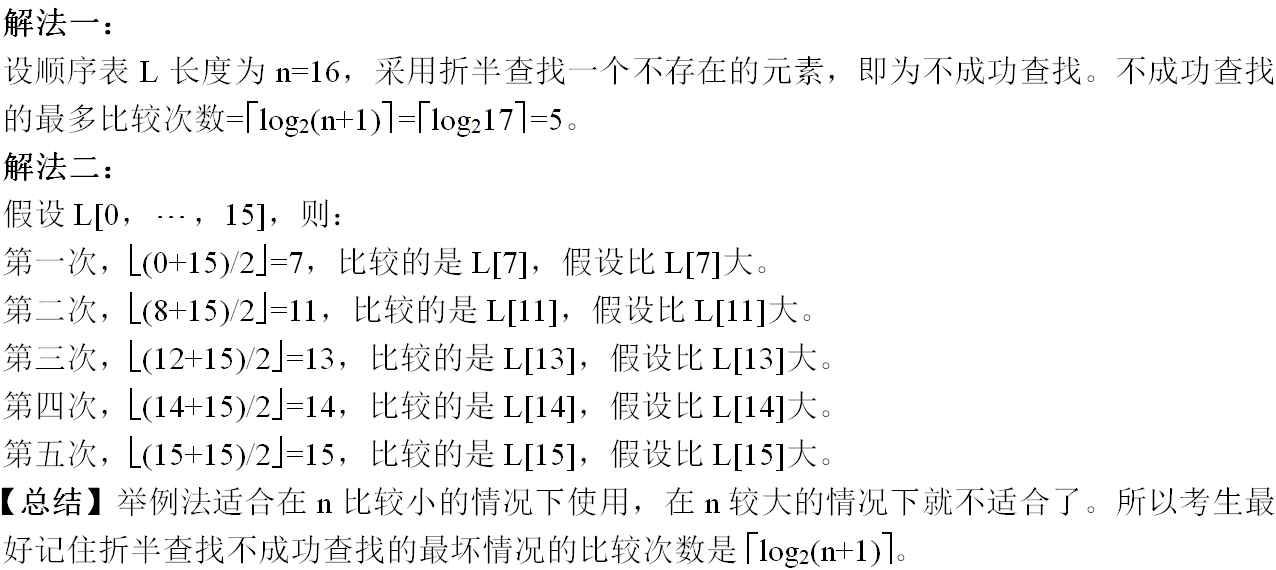
\includegraphics[width=3.46875in,height=1.55208in]{computerassets/FF39BAA734C32BA5A7D30035B50F1E93.png}
\end{solution}
\question (中南大学,2004年)若在线性表中采用折半查找法查找元素,则该线性表应为(
)
\par\twoch{元素按值有序}{\textcolor{red}{元素按值有序,且采用顺序存储结构}}{元素按值有序,且采用链式存储结构}{采用顺序存储结构}
\begin{solution}考察折半查找的概念,折半查找必须要求是元素有序,并且能支持随机访问
\end{solution}
\question (青岛大学,2004年)对长度为10的有序表进行二分查找(折半查找),在等概率的情况下,查找成功的平均查找长度(ASL)为(
)
\par\twoch{3.2}{1.7}{\textcolor{red}{2.9}}{不确定}
\begin{solution}分别列出查找每一个元素所需要的比较次数为3,2,3,4,1,3,4,2,3,4,又因为是等概率,可以求出平均查找长度是(3+2+3+4+1+3+4+2+3+4)/10=2.9
\end{solution}
\question (中科院)设有100个元素,用二分法查找时,最大比较次数是( )
\par\twoch{25}{50}{10}{\textcolor{red}{7}}
\begin{solution}最大比较次数等于折半查找判定树的高度,可计算出判定树的高度为7。
\end{solution}
\question (中科院)在顺序表\{3,6,8,10,12,15,16,18,21,25,30\}中,用二分法查找关键字11,所需的关键字比较次数为(
)
\par\twoch{2}{3}{\textcolor{red}{4}}{5}
\begin{solution}经过4次比较,分别是15,8,10,12,最后发现关键字不在序列中。
\end{solution}
\question (华中科技大学,2005年)折半查找有序表(5,8,10,22,36,50,53,88),若查找元素70,则需要依次与表中元素(关键字)(
)进行比较,查找结果是``失败''
\par\twoch{36,53}{\textcolor{red}{22,50,53,88}}{36,53,88}{22,53,88}
\begin{solution}折半查找的方式如下:如果当前的元素总数为奇数,则查找中间那个元素;如果当前元素总数为偶数,则查找中间考前的一个元素
\end{solution}
